\let\negmedspace\undefined
\let\negthickspace\undefined
\documentclass[journal]{IEEEtran}
\usepackage[a5paper, margin=10mm, onecolumn]{geometry}
%\usepackage{lmodern} 
\usepackage{tfrupee} 

\setlength{\headheight}{1cm} 
\setlength{\headsep}{0mm}     

\usepackage{gvv-book}
\usepackage{gvv}
\usepackage{cite}
\usepackage{amsmath,amssymb,amsfonts,amsthm}
\usepackage{algorithmic}
\usepackage{graphicx}
\usepackage{textcomp}
\usepackage{xcolor}
\usepackage{txfonts}
\usepackage{listings}
\usepackage{enumitem}
\usepackage{mathtools}
\usepackage{gensymb}
\usepackage{comment}
\usepackage[breaklinks=true]{hyperref}
\usepackage{tkz-euclide} 
\usepackage{listings}                                        
\def\inputGnumericTable{}                                 
\usepackage[latin1]{inputenc}                                
\usepackage{color}                                            
\usepackage{array}                                            
\usepackage{longtable}                                       
\usepackage{calc}                                             
\usepackage{multirow}                                         
\usepackage{hhline}                                           
\usepackage{ifthen}                                           
\usepackage{lscape}

\begin{document}

\bibliographystyle{IEEEtran}
\vspace{3cm}

\title{4.7.64}
\author{AI25BTECH11003 - Bhavesh Gaikwad}
{\let\newpage\relax\maketitle}

\renewcommand{\thefigure}{\theenumi}
\renewcommand{\thetable}{\theenumi}
\setlength{\intextsep}{10pt} 


\numberwithin{equation}{enumi}
\numberwithin{figure}{enumi}
\renewcommand{\thetable}{\theenumi}


\textbf{Question}: Find the distance between the point $\vec{P}$(6, 5, 9) and the plane determined by the points $\vec{A}$(3, -1, 2), $\vec{B}$(5, 2, 4) and $\vec{C}$(-1, -1, 6). \\


\solution
Let the Equation of the Plane be $\vec{n}^\top\vec{x}$ = 1.\\

Since, $\vec{A}, \, \vec{B}, \, \vec{C}$ lie on the Plane.

\begin{equation}
    \therefore \, \vec{n}^\top\vec{A}=1, \, \vec{n}^\top\vec{B}=1,  \, \vec{n}^\top\vec{C}=1
\end{equation}

\begin{center}
    OR
\end{center}

\begin{equation}
    \vec{A}^\top\vec{n}=1, \, \vec{B}^\top\vec{n}=1, \, \vec{C}^\top\vec{n}=1
\end{equation}

Let $\vec{n} = \myvec{n_1 \\ n_2 \\ n_3}$

From Equation 0.2,
\begin{equation}
    (\vec{A} \, \vec{B} \, \vec{C})^\top \vec{n}=1
\end{equation}

\begin{equation}
\myvec{3 & -1 & 2 \\ 5 & 2 & 4\\ -1 & -1 & 6}\vec{n} = 1
\end{equation}


From Equation 0.4,
\begin{equation}
\therefore \, \text{The Equation of the Plane is: } \dfrac{1}{19}\myvec{3 & -4 & 3}\vec{x} = 1
\end{equation}\\

The Distance of Point from a Plane is given by the formula:
\begin{equation}
    d = \dfrac{\norm{\vec{n}^\top\vec{Q}-1}}{\norm{\vec{n}}}
\end{equation}

Let $d$ be the distance between Point $\vec{P}$ and the Plane.
\begin{equation}
    Then, \, \, d = \dfrac{\norm{\vec{n}^\top\vec{P}-1}}{\norm{\vec{n}}}
\end{equation}

\begin{equation}
    d= \dfrac{\norm{\frac{18-20+27}{19}-1}}{(\frac{\sqrt{34}}{19})}
\end{equation}

\begin{equation}
\therefore \, d = \dfrac{3\sqrt{34}}{17}    
\end{equation}

\begin{align}
    \boxed{\text{The Distance between the Plane and } \vec{P} \, is \, \dfrac{3\sqrt{34}}{17} \, units.}
\end{align}

\begin{figure}[htbp]
    \centering
    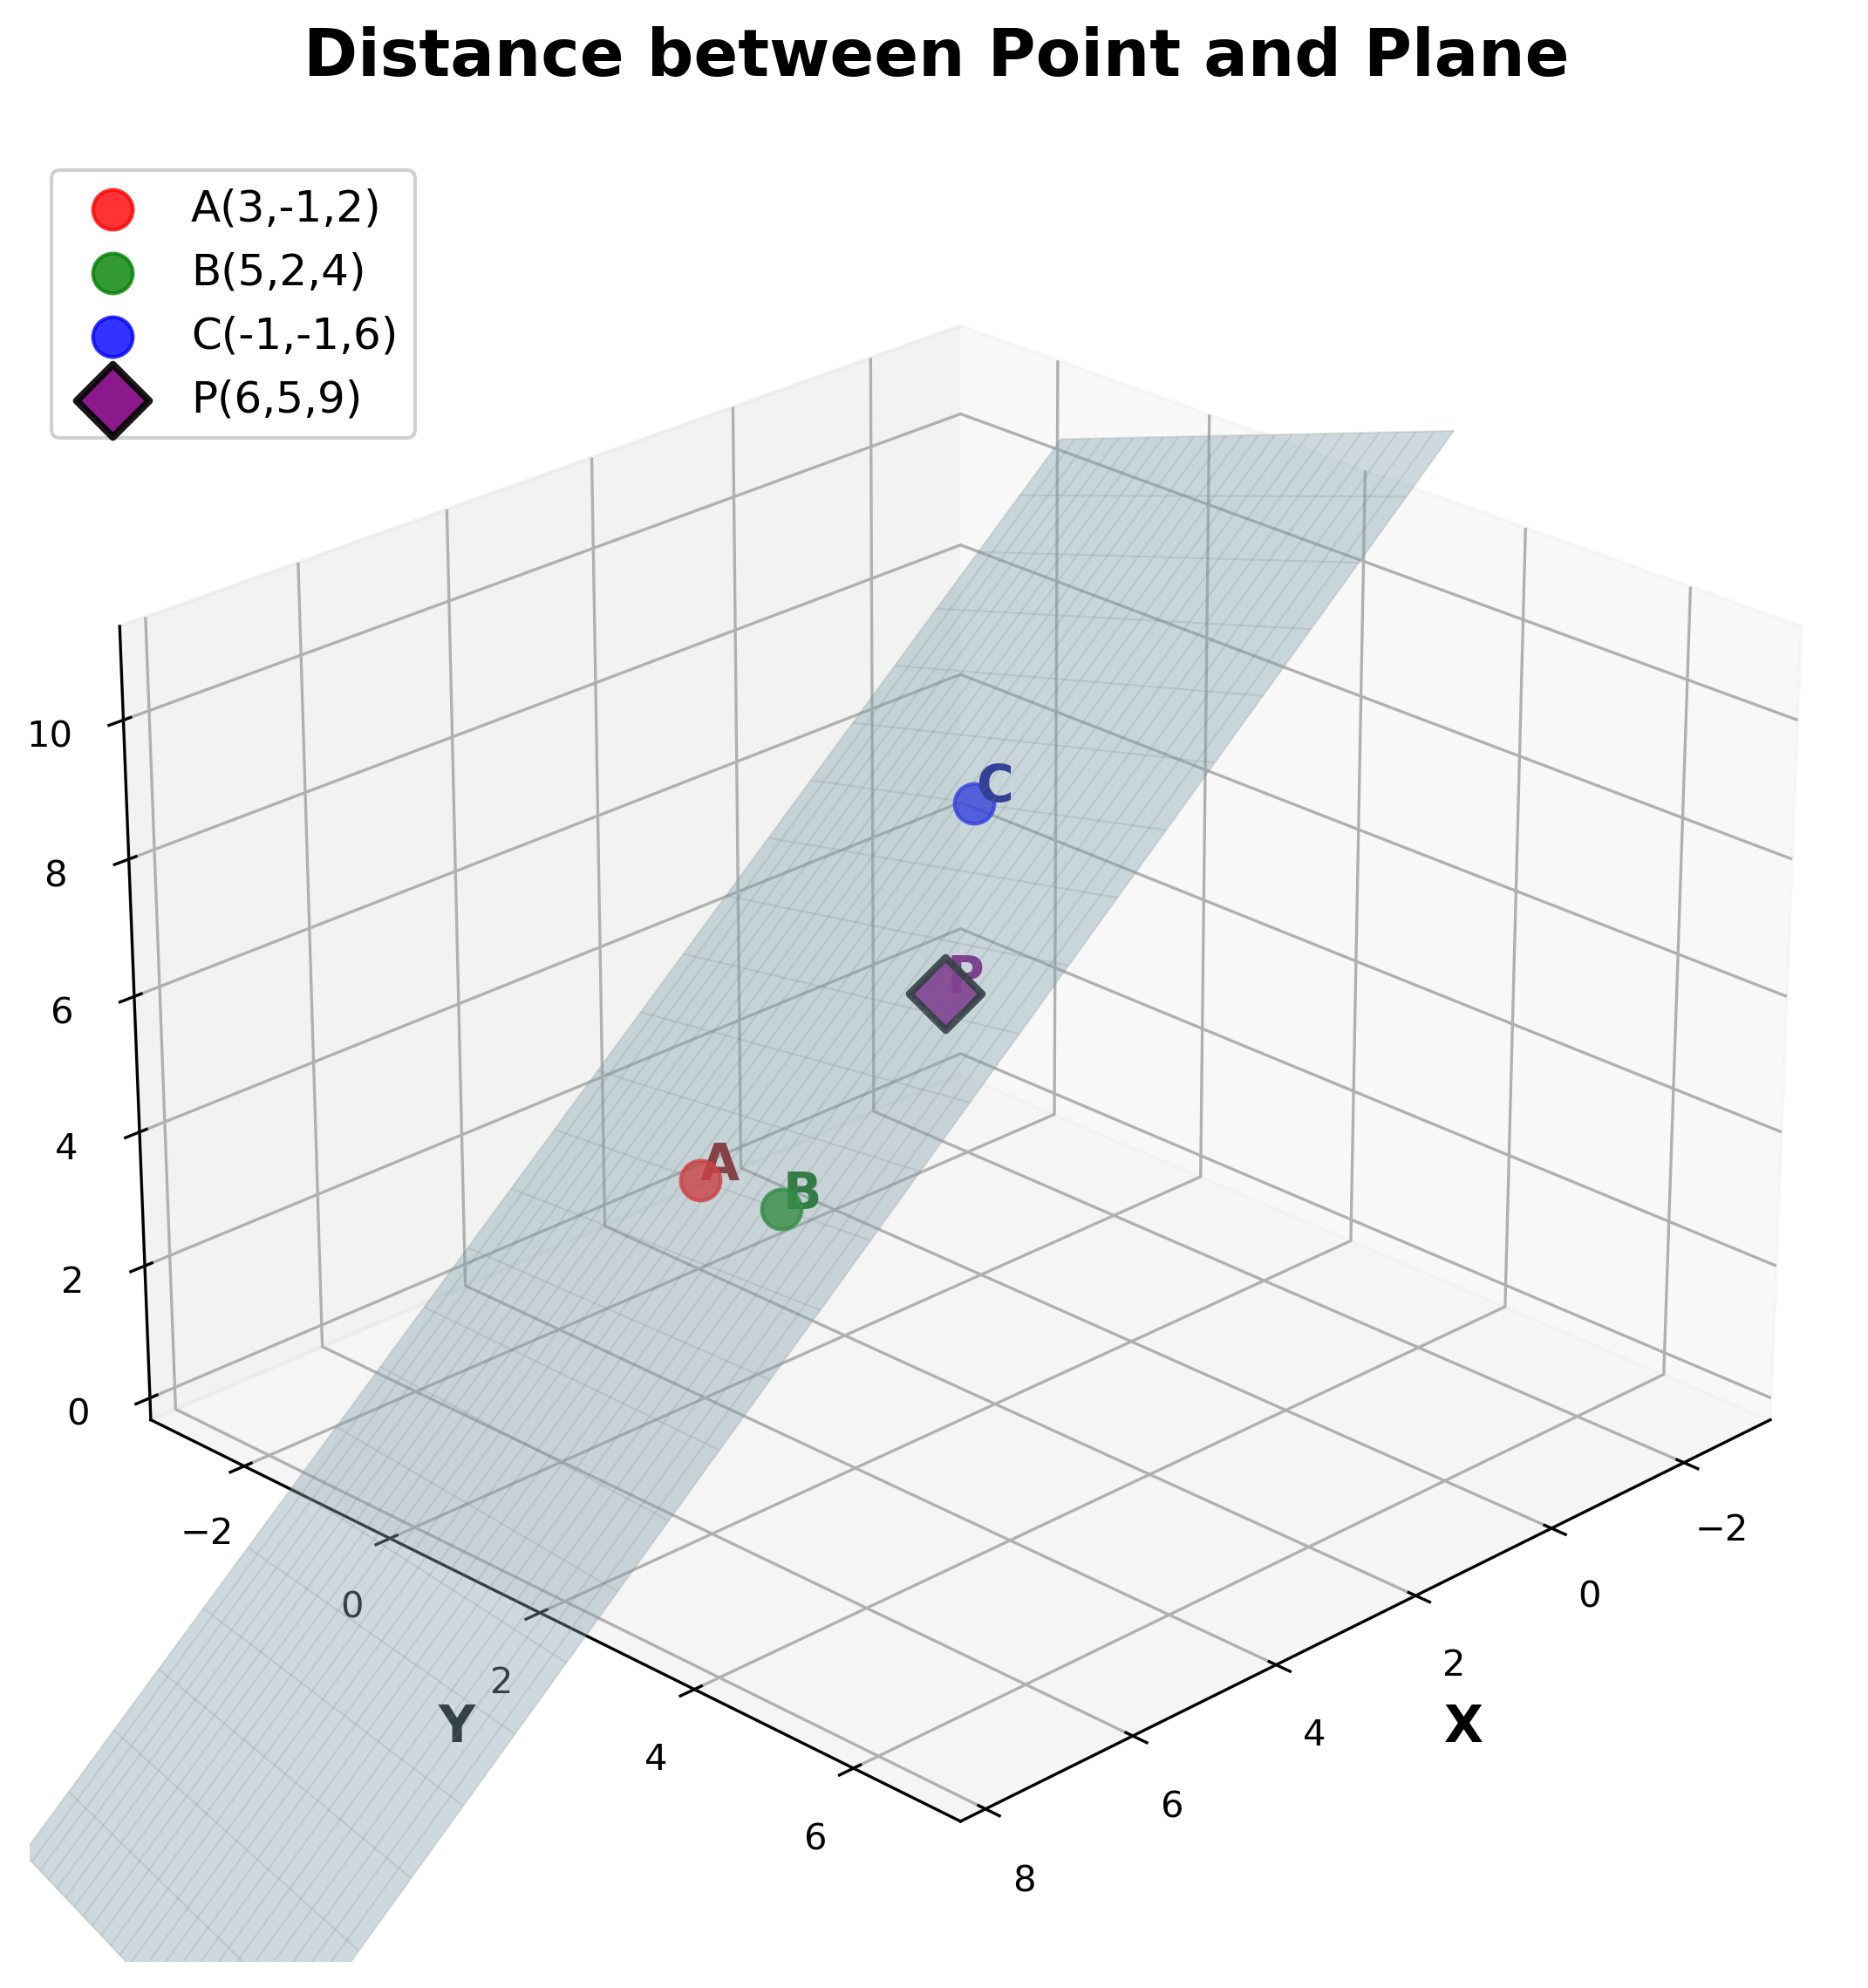
\includegraphics[width=0.95\columnwidth]{figs/fig1.png}
    \caption{Plane}
    \label{fig:fig/fig1.png}
\end{figure}
\end{document}  
